\documentclass[10pt,aspectratio=169]{beamer}
\graphicspath{ {images/} }
% --- pdflatex-safe font & micro-typography ---
\usepackage[T1]{fontenc}
\usepackage[utf8]{inputenc}
\usepackage{lmodern}
\usepackage{microtype}

\usepackage{tikz}
\usetikzlibrary{arrows.meta}

% --- math & symbols ---
\usepackage{amsmath,amssymb,mathtools,bm}

% --- hyperlinks (Beamer already loads hyperref; this is safe) ---
\hypersetup{hidelinks}

% --- theme ---
\usetheme[numbering=fraction]{metropolis}

\usepackage{pgfpages} % for notes layouts

% --- bibliography ---
\usepackage[round,authoryear]{natbib}

% --- Choose ONE of these toggles when compiling ---
% \setbeameroption{hide notes}                        % audience version (default)
% \setbeameroption{show notes}                        % notes printed under each slide
% \setbeameroption{show only notes}                   % notes-only PDF (for printing)
% \setbeameroption{show notes on second screen=right} % slide + notes side-by-side

% --- shortcuts ---
\newcommand{\E}{\mathbb{E}}
\newcommand{\R}{\mathbb{R}}
\newcommand{\btheta}{\boldsymbol{\theta}}
\newcommand{\bx}{\boldsymbol{x}}
\setbeamercovered{transparent}
% --- title info ---
\title{Training and generalization in overparameterized neural networks}
\subtitle{Stage 1 review}
\author{Shreyas Kalvankar}
\institute{TU Delft}
\date{\today}

\begin{document}

\maketitle

% -----------------------------------------------------------
% AGENDA SLIDE (visual blocks)
% -----------------------------------------------------------
\begin{frame}{Agenda}

	\textbf{Agenda}
	\begin{enumerate}
		\item Introduction \& Problem setup
		\item Related work
		\item Research Questions \& Objectives
		\item Preliminary observations
		\item Planned work \& Discussions
	\end{enumerate}

\end{frame}

\begin{frame}{Introduction \& Problem setup}
	\textbf{Problem setup: Empirical Risk Minimization}
	\begin{itemize}
		\item Data: $n$ observations $\{(x_i, y_i)\}_{i=1}^n$, with inputs $ x_i \in \mathbb{R}^d$ and targets $y_i \in \mathbb{R}$  (stacked as $X \in \mathbb{R}^{d \times n}, y \in \mathbb{R}^n$).
		      \pause
		\item Prediction function: $f(x) \in \R$
		\item Task: Find the function $f^*$
		      \pause
		\item Objective: that minimizes the empirical risk:
		      \pause
		      \only<4>{$\mathcal{L}(f) = \displaystyle\sum_{i=1}^{n} d(f(x_i), y_i) = \displaystyle\sum_{i=1}^{n}(f(x_i) - y_i)^2$}
		      \only<5>{$\mathcal{L}(f) = d(f_\theta(X), Y) = \|(f(X) - y)\|^2$}
	\end{itemize}

\end{frame}

\begin{frame}[t]{Introduction \& Problem setup}
	\centering
	\begin{minipage}{0.8\textwidth} % Wraps the text in a narrower box
		In order to minimize the empirical risk we consider a family of parameterized functions
		$f_\theta: \R^d \to R$:
		\begin{itemize}
			\item Linear Networks: $f_\theta(x) = x^\top \theta$
			      \pause
			\item Neural Networks: $f_\theta(x) = $
		\end{itemize}
	\end{minipage}
	\begin{tikzpicture}[remember picture, overlay]
		\node<2->[anchor=south east, xshift=-5cm, yshift=1.7cm]
		at (current page.south east)
		{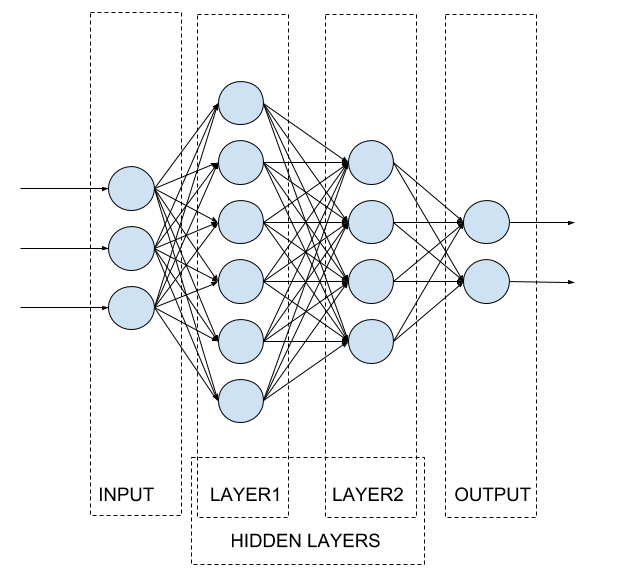
\includegraphics[width=4.5cm]{neural-network}};
	\end{tikzpicture}

	\begin{tikzpicture}[remember picture, overlay]

		% 1. RED ARROW (Left, pointing UP)
		% Adjust 'xshift' to move left/right, 'yshift' to move up/down
		\draw<4->[red!80!black, line width=1.5mm, -{Triangle[width=3mm,length=3mm]}]
		([xshift=2cm, yshift=-5cm]current page.north west) --
		([xshift=2cm, yshift=-3cm]current page.north west)
		node[midway, left=0.2cm, align=right, font=\bfseries\small] {Simplicity\\of\\analysis};

		% 2. BLUE ARROW (Right, pointing DOWN)
		\draw<3->[blue!80!black, line width=1.5mm, -{Triangle[width=3mm,length=3mm]}]
		([xshift=-3cm, yshift=-3cm]current page.north east) --
		([xshift=-3cm, yshift=-5cm]current page.north east)
		node[midway, right=0.2cm, align=left, font=\bfseries\small] {Expressivity\\power};

	\end{tikzpicture}
\end{frame}

\begin{frame}{Why Analyze Training Dynamics?}

	\begin{itemize}
		\item Neural networks are trained using gradient-based methods on high-dimensional, non-convex objectives.
		      \pause
		\item Understanding \textbf{training dynamics} is key to explaining convergence behavior and generalization.
		      \pause
		\item However, for nonlinear networks like neural networks, these dynamics are difficult to characterize analytically.
	\end{itemize}

\end{frame}

\begin{frame}[t]{Why Are Nonlinear Dynamics Hard?}

	\begin{itemize}
		\item For linear models, gradient descent induces a linear dynamical system where convergence can
		      be explained by the spectrum of the covariance matrix (operator) $XX^\top$.
			      {\footnotesize
				      \[
					      f_w(x) = x^\top w \qquad \qquad \qquad \dot{w_t} = -\nabla_w\mathcal{L}(w_t) = Xy - XX^\top w_t
				      \]
			      }
		      \vspace{-2em}
		      \pause
		\item Introducing depth to linear models already leads to coupled, nonlinear dynamics with no general closed-form solution.
		      \begin{columns}[T,onlytextwidth]
			      % ---- Left column: image or equation ----
			      \begin{column}{0.35\textwidth}
				      \centering
				      {\footnotesize
					      \[
						      f_{v,W}(x) = (Wx)^\top v
					      \]
				      }
				      % or:
				      % \includegraphics[width=\linewidth]{nonlinear_schematic.pdf}
			      \end{column}
			      % ---- Right column: gradient flow ----
			      \begin{column}{0.65\textwidth}
				      {\footnotesize
					      \[
						      \begin{aligned}
							      \dot v_t = -\nabla_v \mathcal{L}(v_t,W_t)
							       & = W_t X \bigl(y - X^\top W_t^\top v_t\bigr)             \\
							      \dot W_t = -\nabla_W \mathcal{L}(v_t,W_t)
							       & = v_t \bigl(y - X^\top W_t^\top v_t\bigr)^\top X^\top .
						      \end{aligned}
					      \]
				      }
			      \end{column}
		      \end{columns}
		      \pause
		\item Adding nonlinear activations mixes matrix products with elementwise nonlinearities.
		      \begin{columns}[T,onlytextwidth]
			      % ---- Left column: image or equation ----
			      \begin{column}{0.35\textwidth}
				      \centering
				      {\footnotesize
					      \[
						      f_{v,W}(x) = \phi(Wx)^\top v
					      \]
				      }
				      % or:
				      % \includegraphics[width=\linewidth]{nonlinear_schematic.pdf}
			      \end{column}
			      % ---- Right column: gradient flow ----
			      \begin{column}{0.65\textwidth}
				      {\footnotesize
					      \[
						      \begin{aligned}
							      \dot v_t
							       & = \phi(W_t X)\bigl(y - \phi(W_t X)^\top v_t\bigr),                        \\[-0.4em]
							      \dot W_t
							       & = \big(\phi'(W_t X)\odot v_t (y - \phi(W_t X)^\top v_t)^\top\big)X^\top .
						      \end{aligned}
					      \]
				      }
			      \end{column}
		      \end{columns}
		      \pause
		\item We don't know of any mathematical tools to analyse such systems.
	\end{itemize}

\end{frame}

\begin{frame}
	\huge Related work
\end{frame}

\begin{frame}[t]{Solution: Take limits!}

	\begin{tikzpicture}[remember picture, overlay]
		\node<2->[anchor=south east, xshift=-8.5cm, yshift=1cm]
		at (current page.south east)
		{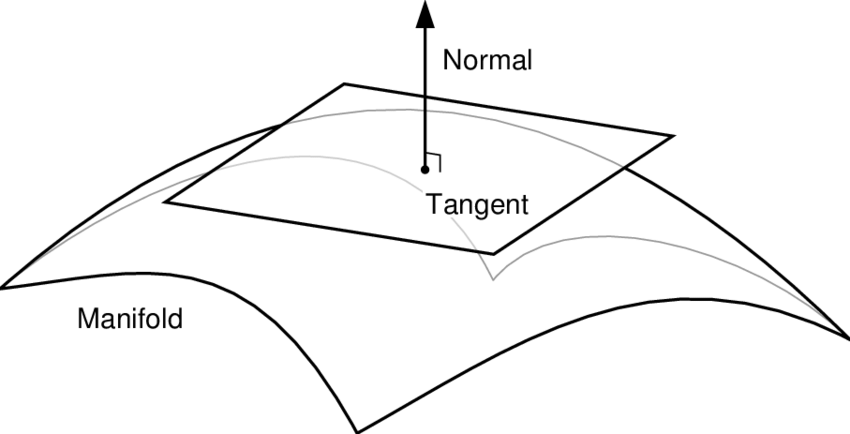
\includegraphics[width=4.5cm]{tangent-plane}};
		\node<4->[anchor=south east, xshift=-2.5cm, yshift=1cm]
		at (current page.south east)
		{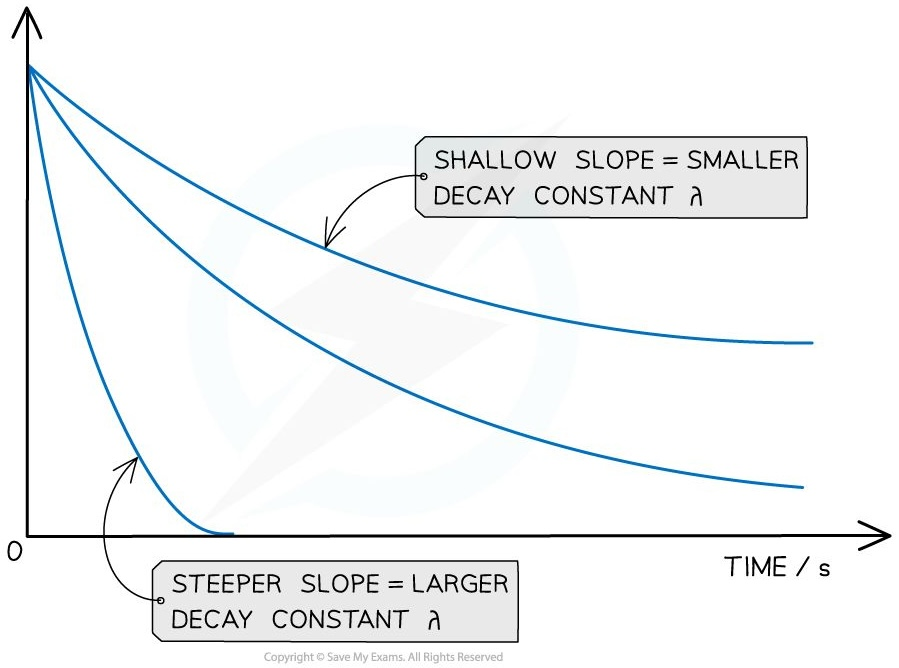
\includegraphics[width=4.5cm]{decay}};
	\end{tikzpicture}
	\begin{itemize}
		\item In the infinite-width limit, neural network training can be linearized around initialization.
		      \pause
		\item The resulting dynamics are linear and governed by the \textbf{Neural Tangent Kernel (NTK)}.
		      \pause
		\item Training becomes equivalent to kernel gradient descent with a fixed kernel.
		      \pause
		\item Convergence behavior is governed by the spectrum of the NTK operator.
	\end{itemize}

	\begin{tikzpicture}[remember picture, overlay]
		\node[anchor=south, yshift=0.2cm, text opacity=0.4]
		at (current page.south)
		{\footnotesize Image Sources: DOI:10.1137/S0895479895290954; Katie M., AQA A Level Physics Notes};
	\end{tikzpicture}

\end{frame}

\begin{frame}[t]{Spectral Bias in the NTK Regime}
	\begin{tikzpicture}[remember picture, overlay]
		\node<2->[anchor=south east, xshift=-7cm, yshift=0.5cm]
		at (current page.south east)
		{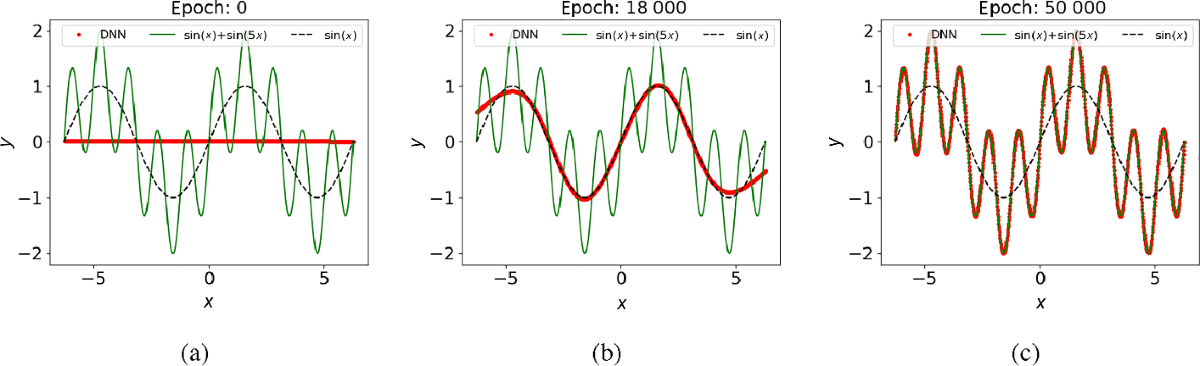
\includegraphics[width=8cm]{spectral-bias}};
		\node<4->[anchor=south east, xshift=-2.5cm, yshift=0.8cm]
		at (current page.south east)
		{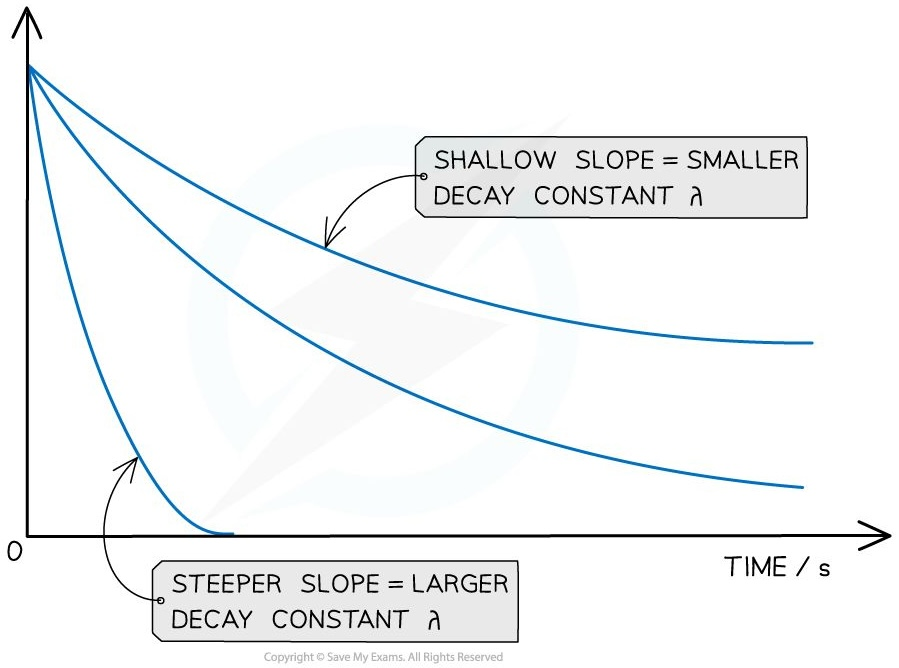
\includegraphics[width=3.3cm]{decay}};
	\end{tikzpicture}
	\begin{itemize}
		\item A well-known empirical phenomenon in neural network training is \textbf{spectral bias}:
		      low-frequency components are learned faster than high-frequency ones.
		      \pause
		\item In the NTK limit, this phenomenon admits a precise theoretical explanation.
		      \pause
		\item For ReLU networks trained on a continuum domain (e.g.\ $[0,2\pi]$),
		      the NTK operator is diagonal in the Fourier basis.
		      \pause
		\item Eigenvalues are ordered by frequency: lower frequencies correspond to larger eigenvalues.
	\end{itemize}
	\begin{tikzpicture}[remember picture, overlay]
		\node[anchor=south, yshift=0.2cm, text opacity=0.4]
		at (current page.south)
		{\footnotesize Image Sources: Overview Spectral Bias in Deep Learning, vol 7;
			Katie M., AQA A Level Physics Notes};
	\end{tikzpicture}

\end{frame}

\begin{frame}{The Gap: Beyond the Ideal NTK}

	\begin{itemize}
		\item Spectral bias is observed empirically in \textbf{finite-width} neural networks.
		      \pause
		\item Existing theoretical results characterize spectral bias in the
		      \textbf{infinite-width, population NTK limit}, where training dynamics are
		      governed by a deterministic integral operator.
		      \pause
		\item While finite-width and finite-sample networks are known to track NTK dynamics to
		      some extent, it remains unclear how
		      \textbf{frequency-wise learning dynamics} are quantitatively affected by
		      finite width and finite sample size.
	\end{itemize}

\end{frame}

\begin{frame}
	\huge Research objective
\end{frame}

\begin{frame}{Common Setting and Assumptions}

	\begin{itemize}
		\item \textbf{Data:} inputs $x(\theta)=(\cos\theta,\sin\theta)$ on $S^1$,
		      sampled uniformly unless stated otherwise.
		\item \textbf{Target functions:} finite Fourier mixtures of the form
		      \[
			      f^\star(\theta)
			      =
			      \sum_{k \in \mathcal{K}} a_k \sin(k\theta),
		      \]
		      with a finite frequency set $\mathcal{K}$ and fixed coefficients.
		\item \textbf{Model:} two-layer ReLU network trained by gradient descent.
		\item \textbf{Training:} fixed learning rate and fixed number of training steps.
	\end{itemize}

\end{frame}

\begin{frame}{Main Research Question}

	\textbf{Main Question.}
	To what extent do the frequency-wise training dynamics predicted by the ideal
	infinite-width, population NTK persist when either the number of training samples
	or the network width is finite?

	\vspace{0.6em}

	\textbf{More precisely:}
	\begin{itemize}
		\item how are the decay rates of individual Fourier components of the training error
		      affected by finite sample size?
		      \pause
		\item how are these frequency-wise dynamics perturbed by finite network width
		      when training population is effectively infinite?
	\end{itemize}

\end{frame}

\begin{frame}{Research Question Q1: Finite-Sample Frequency Dynamics}

	\textbf{Setting.}
	Consider a two-layer ReLU network in the infinite-width NTK regime, with inputs on
	$S^1$ and uniform sampling.
	The population NTK defines a convolution operator $T$ diagonalized by Fourier modes.

	\vspace{0.5em}

	\textbf{Question.}
	What happens to the frequency-wise error decay when the population NTK operator $T$
	is replaced by its finite-sample discretization $T_n$?

	\vspace{0.5em}
	\pause

	\textbf{Approach.}
	We discretize the NTK integral operator via its Mercer decomposition and analyze the
	resulting finite-dimensional linear system governing the evolution of Fourier
	coefficients of the residual.

	\vspace{0.5em}

	\textbf{Focus.}
	We examine how finite sampling affects:
	\begin{itemize}
		\item the rate of decay of error projected onto individual Fourier modes,
		\item deviations from ideal exponential decay,
		\item and interactions between distinct frequency components induced by discretization.
	\end{itemize}

\end{frame}

\begin{frame}{Research Question Q2: Finite-Width Frequency Dynamics}

	\textbf{Setting.}
	Consider a two-layer ReLU network on $S^1$ in a regime where the NTK is approximately
	constant.
	The infinite-width NTK defines a convolution operator $T$ diagonalized by Fourier modes.

	\vspace{0.5em}

	\textbf{Question.}
	What happens to the frequency-wise error decay when the population NTK operator $T$
	is replaced by the random finite-width NTK operator $T^{(m)}$ induced by $m$ neurons?

	\vspace{0.5em}
	\pause

	\textbf{Approach.}
	Treat $T^{(m)}$ as a random perturbation of $T$, project the residual dynamics onto
	Fourier modes, and analyze the resulting coupled linear system for Fourier coefficients.

	\vspace{0.5em}

	\textbf{Focus.}
	We examine how finite width affects:
	\begin{itemize}
		\item the decay of error projected onto individual Fourier modes,
		\item deviations from ideal exponential decay rates,
		\item and mode interactions induced by finite-width NTK.
	\end{itemize}

\end{frame}

\begin{frame}
	\huge Preliminary observations
\end{frame}

\begin{frame}{Spectral Bias on Fourier Mixtures (EXP001)}
	\centering
	\vspace{2mm}
	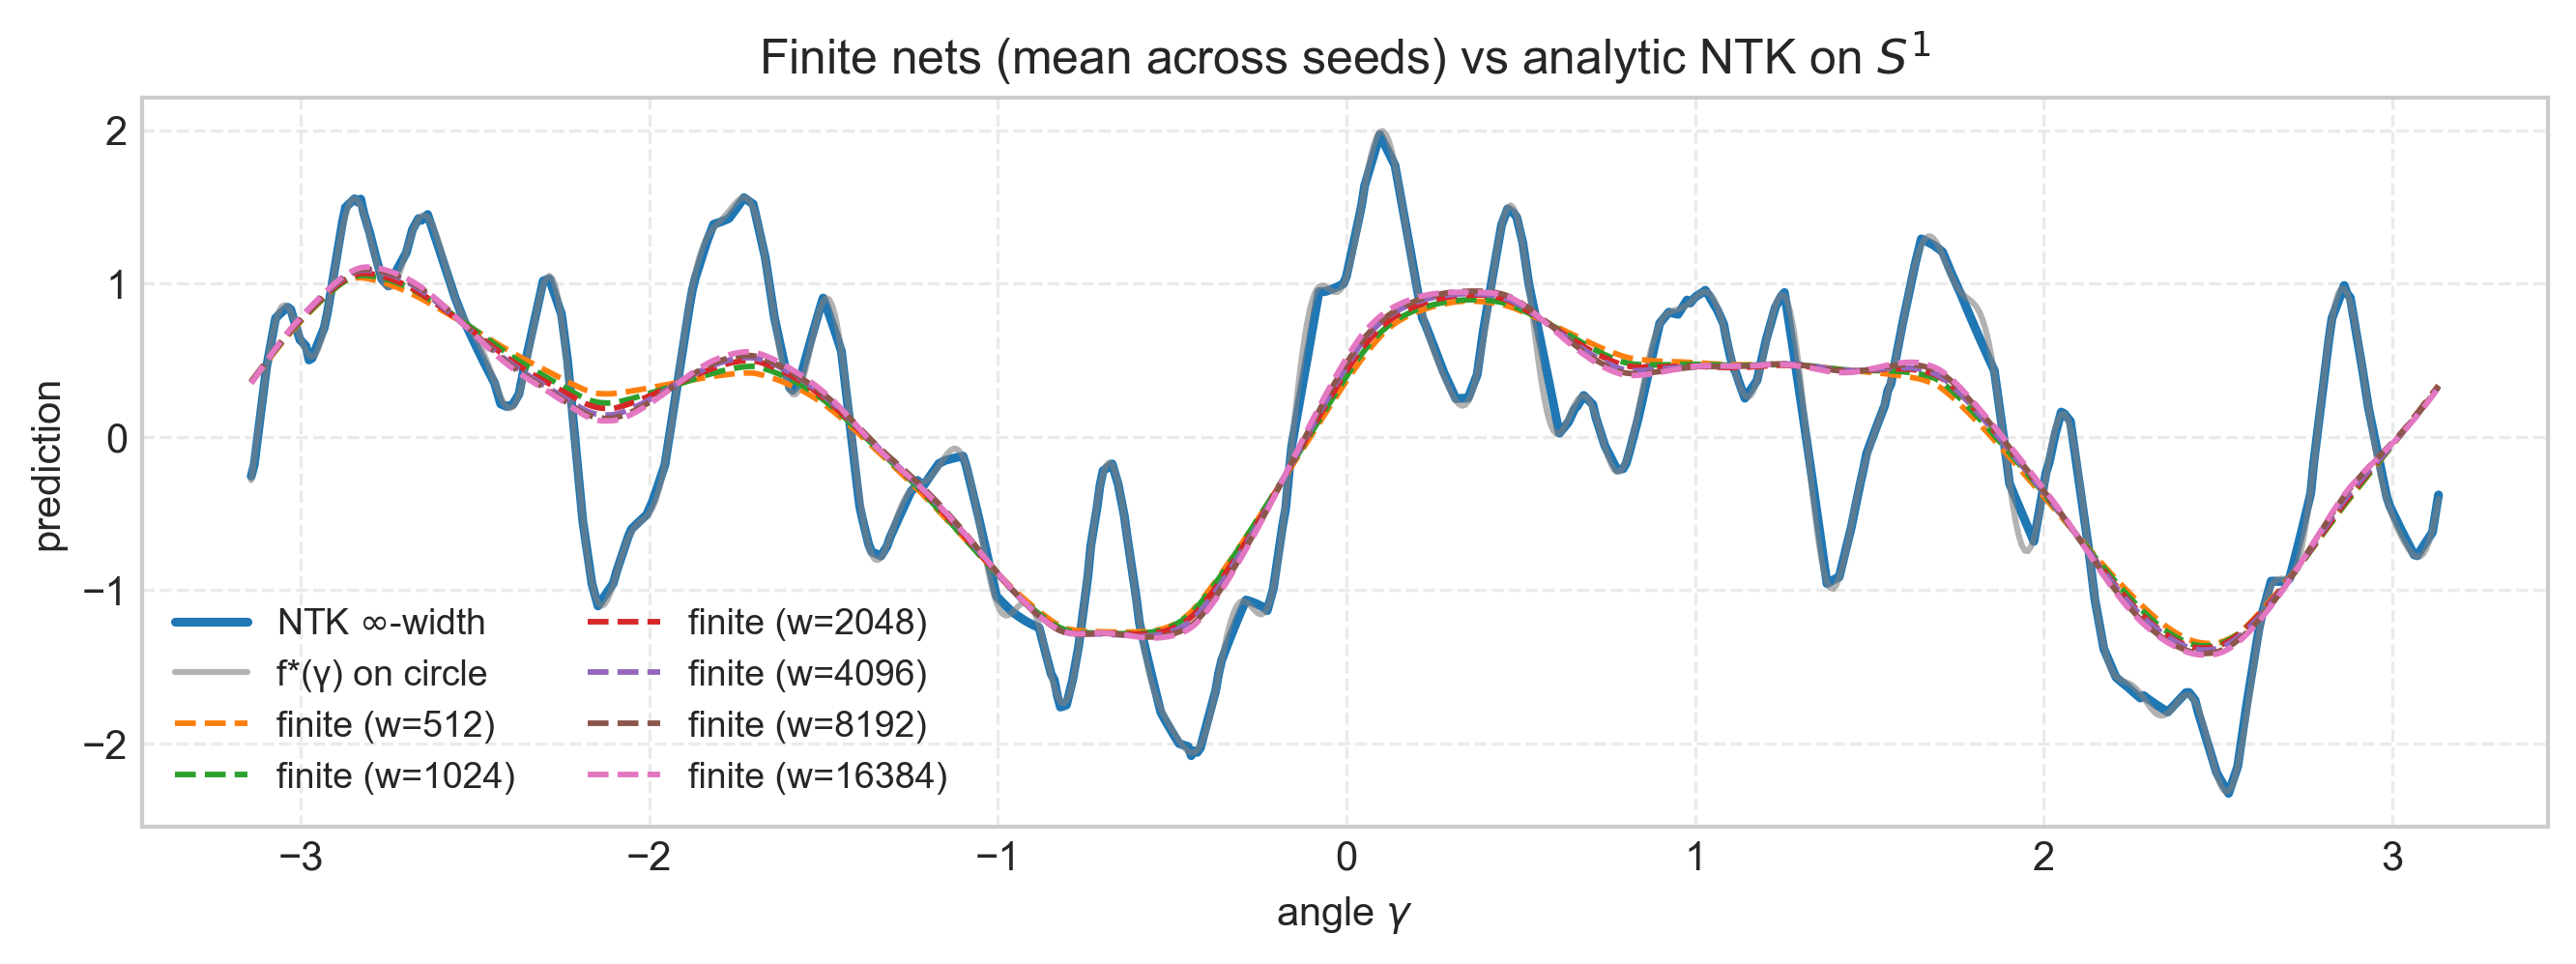
\includegraphics[width=.9\textwidth]{plots/complex-regression/convergence-on-complex-regression-task}
	\\[-1.5mm]\small Learned functions (trained with learning rate = 1e-3, 30k training steps).

	\vspace{0.4em}
	\textbf{Observation.}
	Learned functions are dominated by low frequencies under a fixed training horizon,
	with only weak dependence on width.

	\textbf{Interpretation.}
	High-frequency components converge slowly due to small NTK eigenvalues, motivating frequency-resolved analysis.

\end{frame}

\begin{frame}{Delayed Learning of High Frequencies (EXP001)}
	\vspace{2mm}
	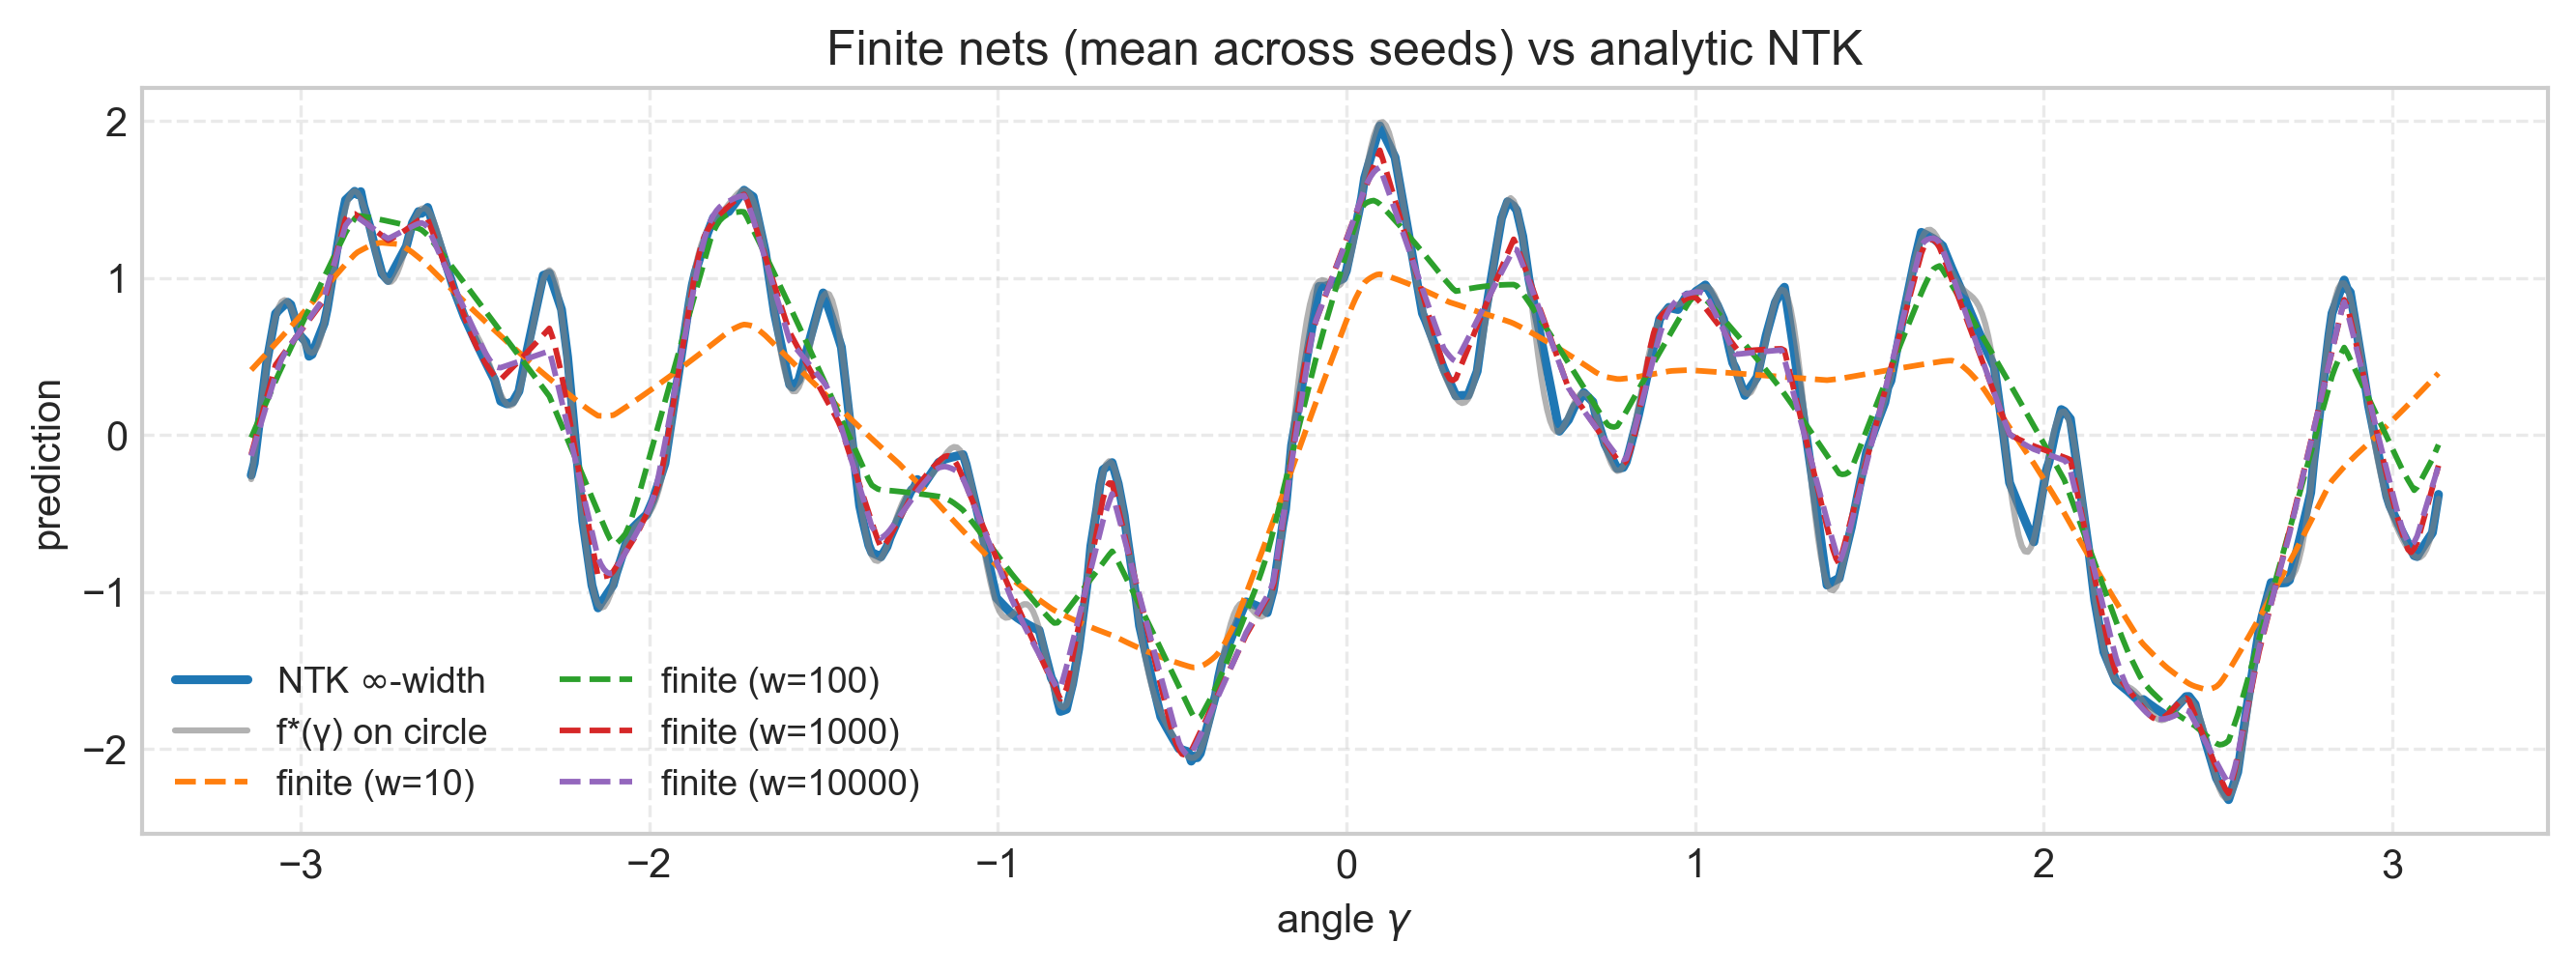
\includegraphics[width=.85\textwidth]{plots/low-width-high-lr-timesteps/convergence-last-low-widths-more-steps-on-simpler-regression-task}
	\\[-1.5mm]\small Learned functions (trained with learning rate = 1, 100k training steps).

	\vspace{0.4em}
	\textbf{Observation.}
	With larger effective training $\eta t$, higher-frequency structure emerges,
	even at small widths.

	\textbf{Interpretation.}
	Spectral bias reflects slow convergence of small-eigenvalue modes,
	not merely representational limits.

\end{frame}

\begin{frame}{Empirical NTK Drift (Low and Mid Widths) (EXP002)}

	\centering
	\begin{minipage}[t]{0.48\textwidth}
		\centering
		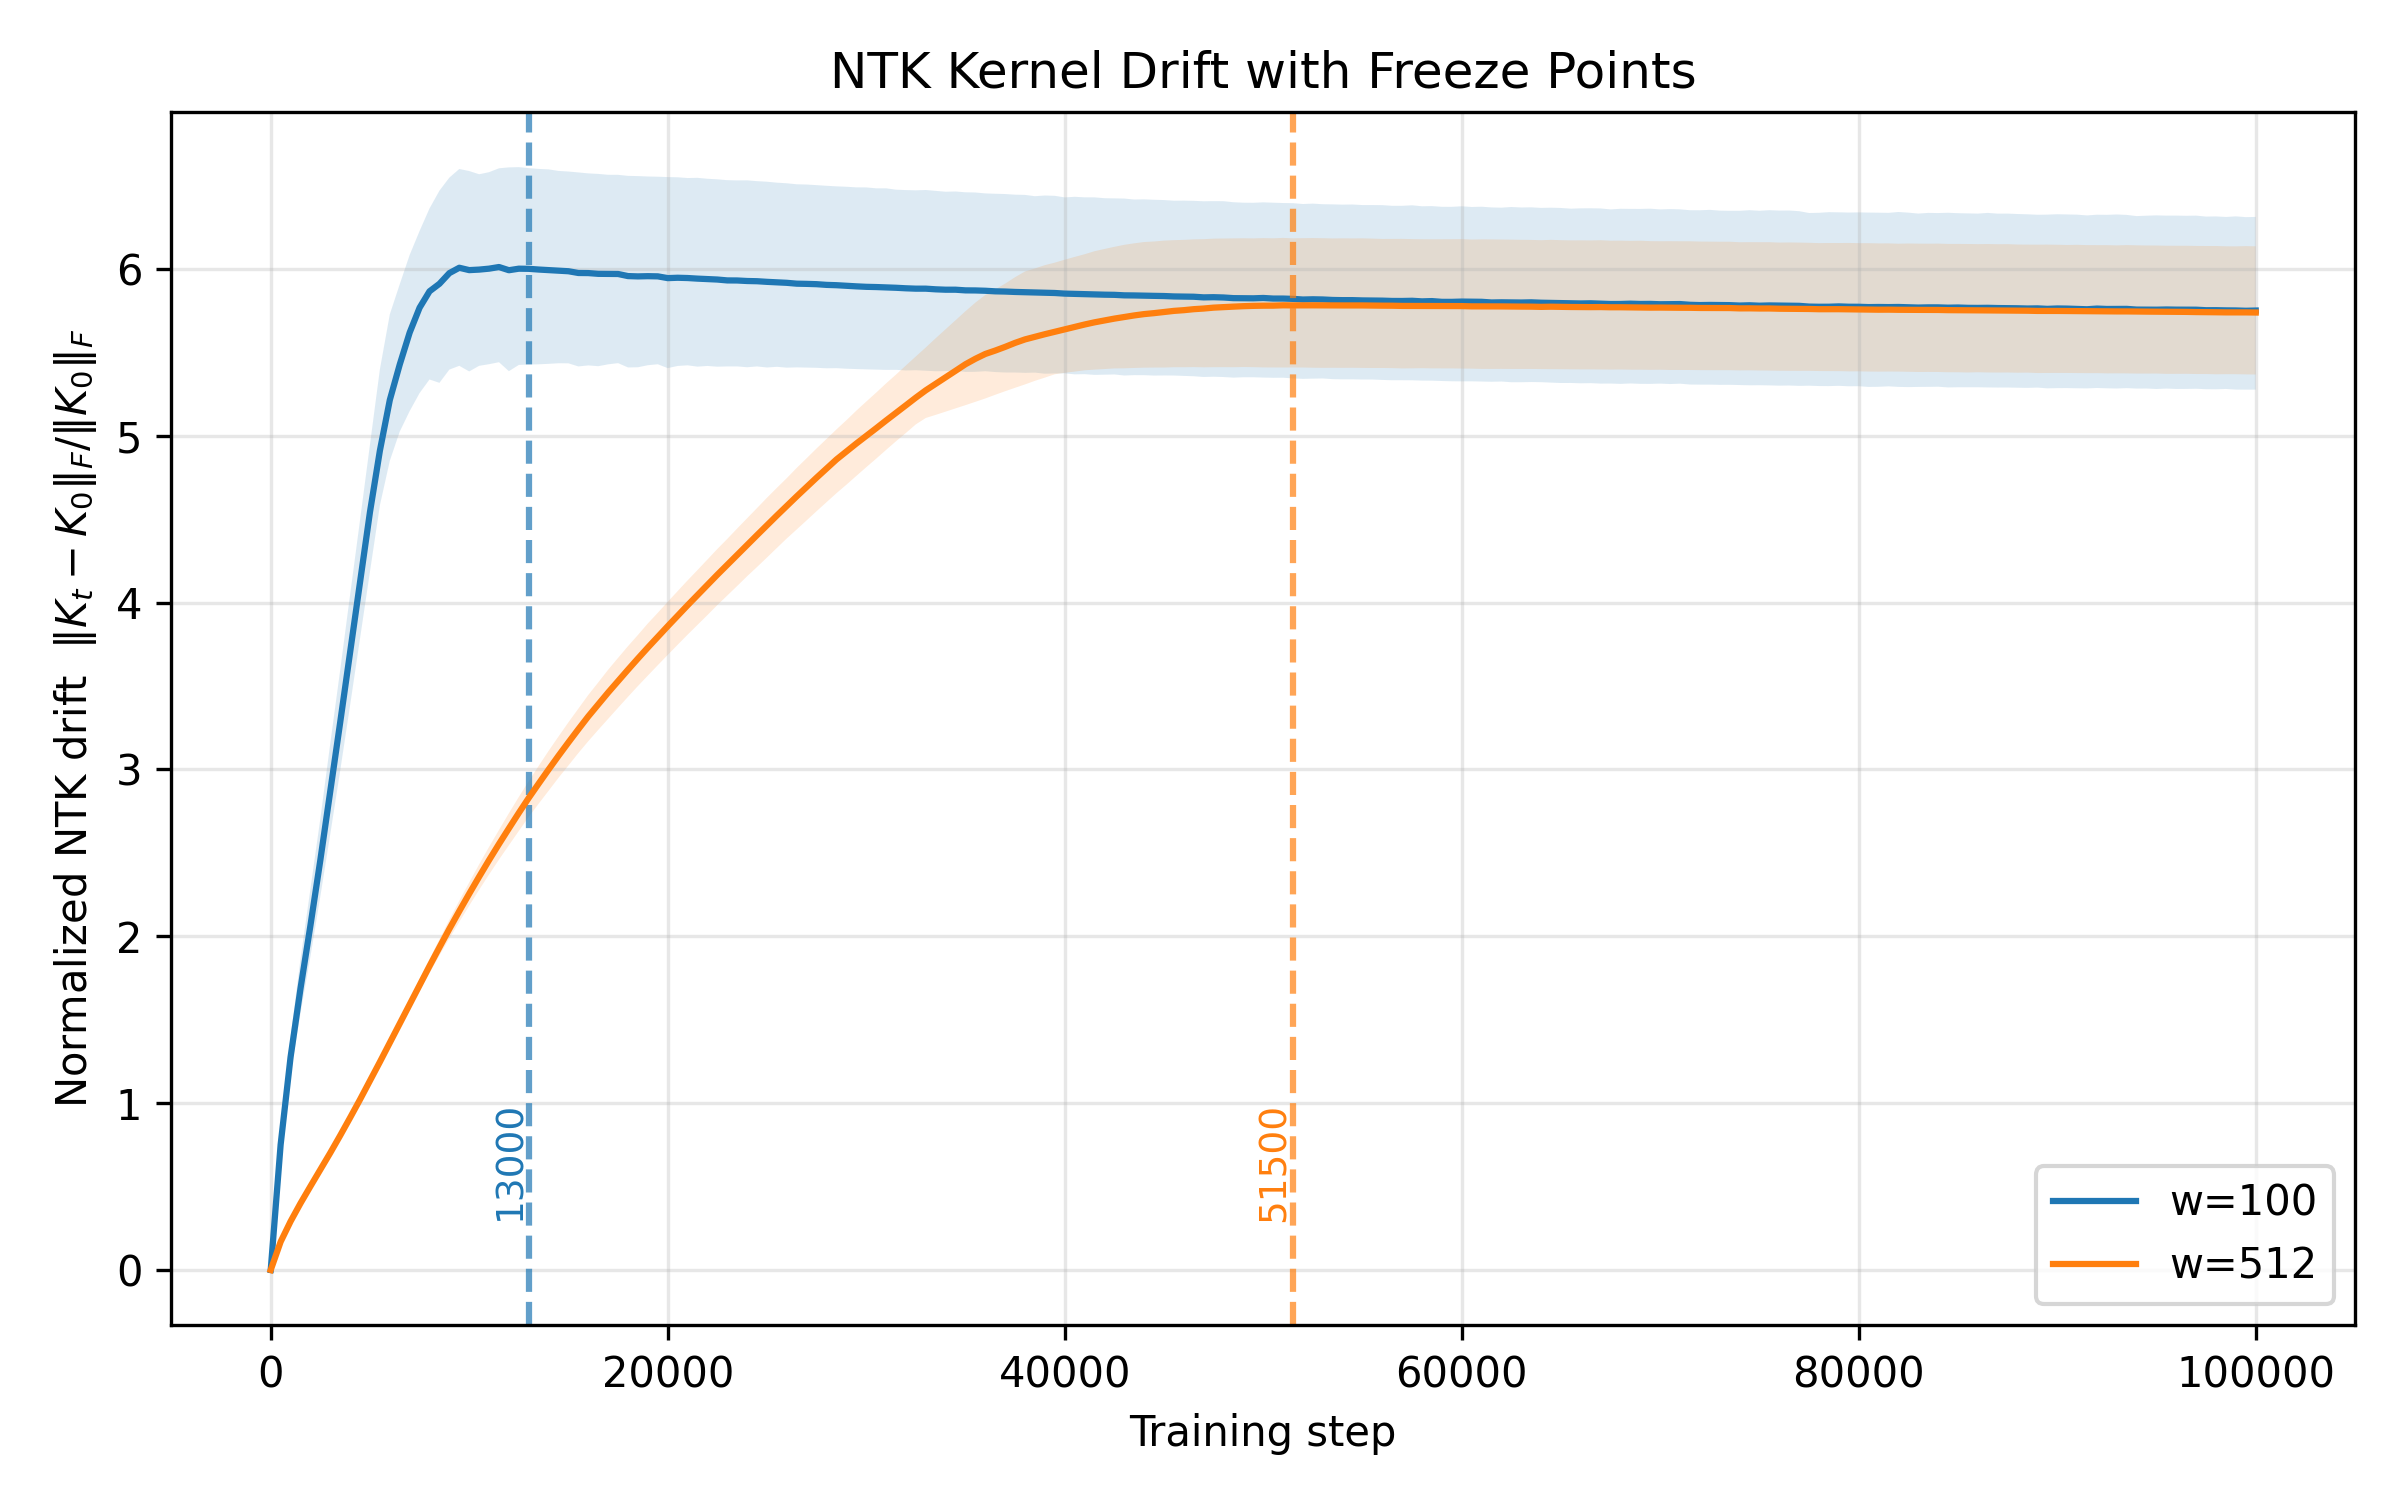
\includegraphics[width=\linewidth]{plots/kernel_drift/kernel_drift_low_widths}
		\\[-1.5mm]\small (a) Low widths.
	\end{minipage}\hfill
	\begin{minipage}[t]{0.48\textwidth}
		\centering
		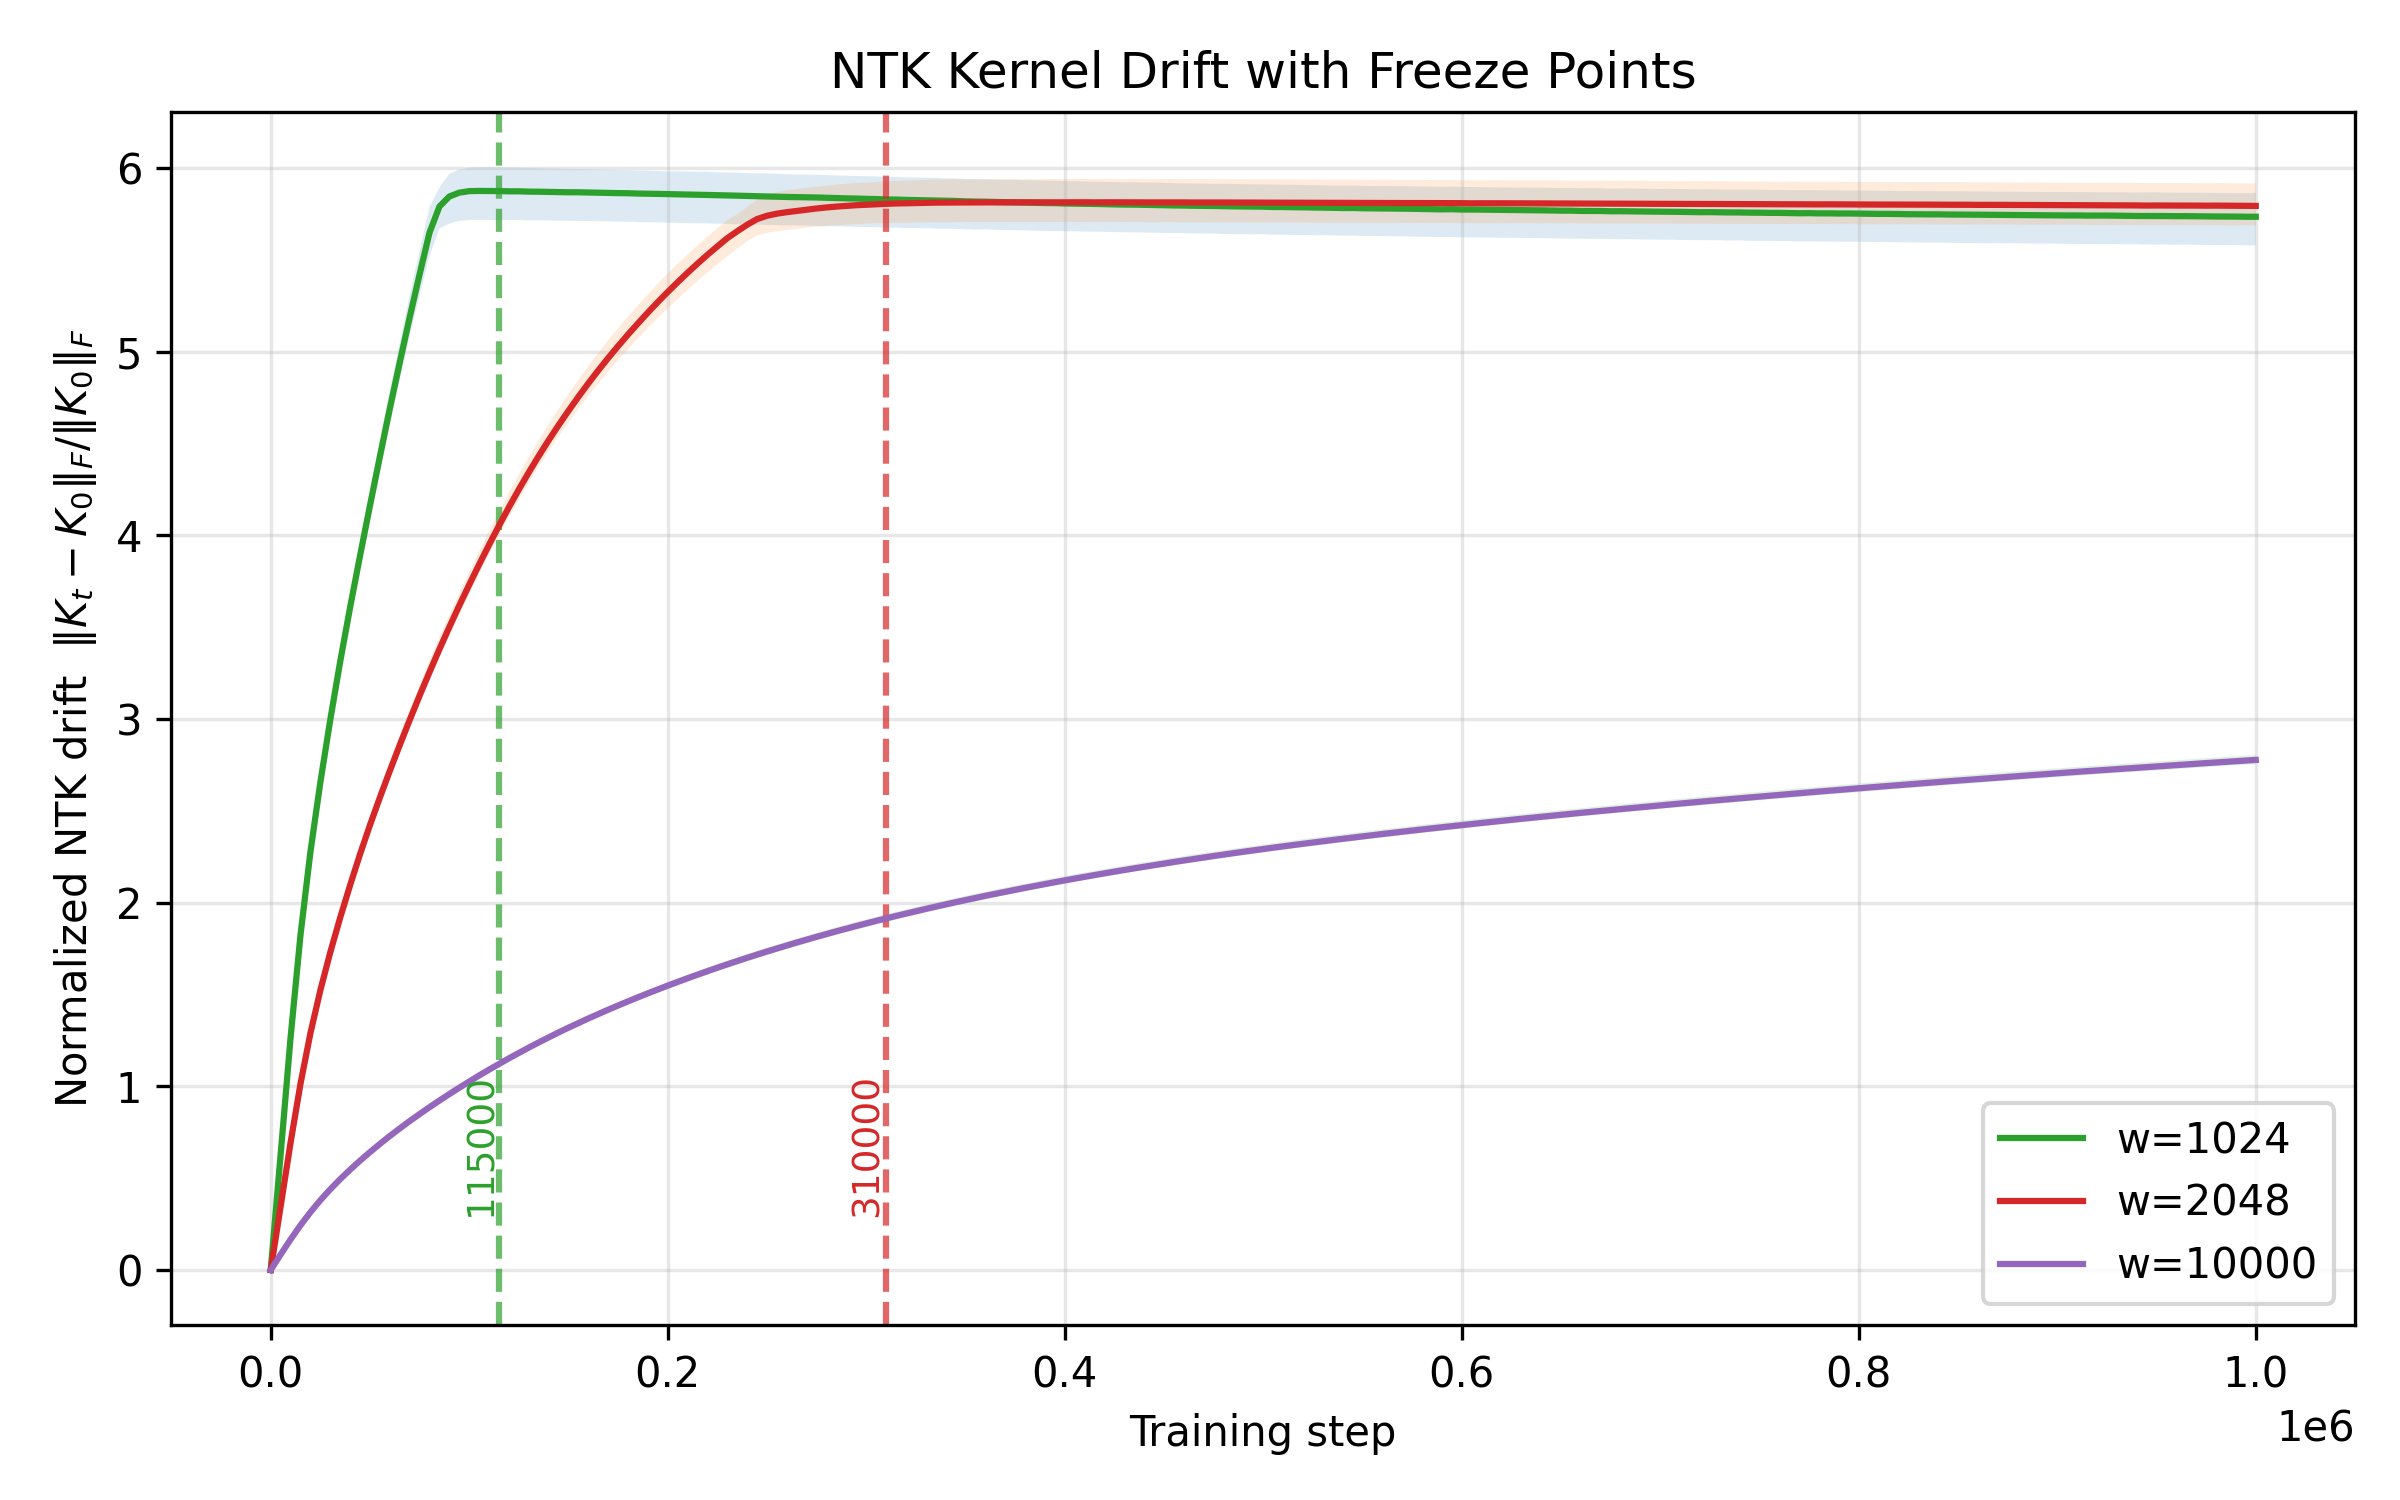
\includegraphics[width=\linewidth]{plots/kernel_drift/kernel_drift_mid_widths}
		\\[-1.5mm]\small (b) Mid widths.
	\end{minipage}

\end{frame}
\begin{frame}{Empirical NTK Drift (High Width) (EXP002)}

	\centering
	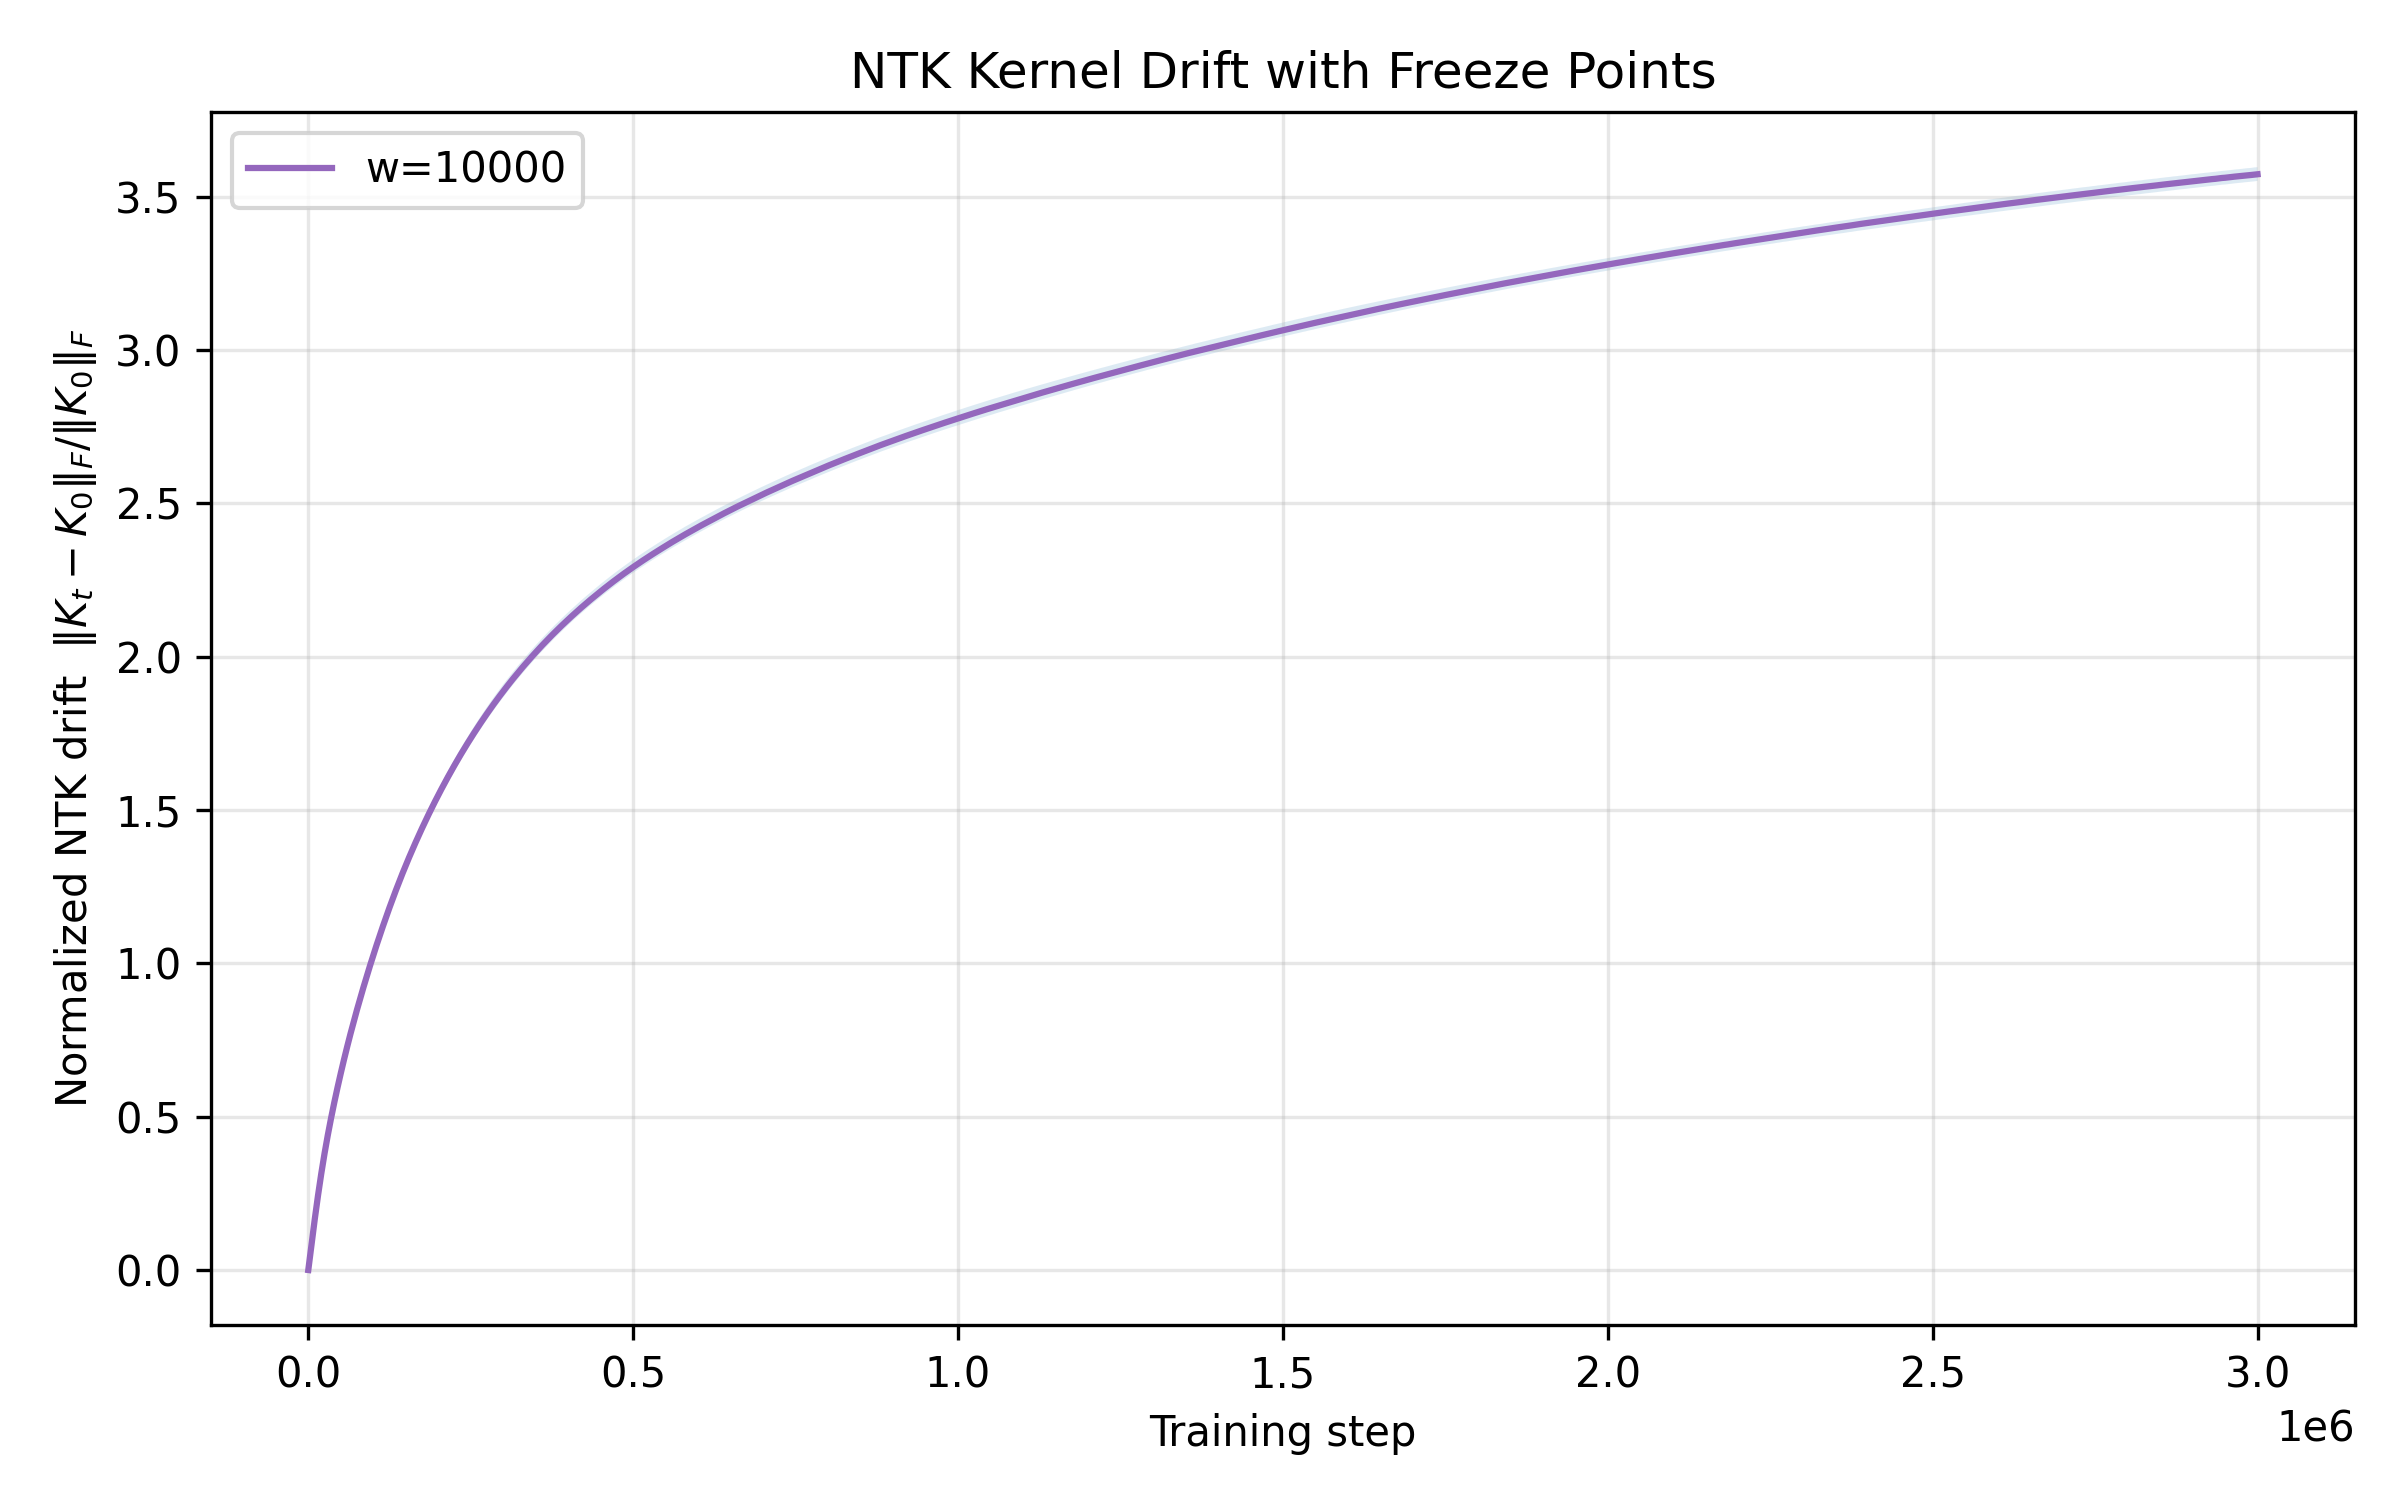
\includegraphics[width=0.6\textwidth]{plots/kernel_drift/kernel_drift_high_widths}
	\\[-1.5mm]\small (c) High width.

\end{frame}


\begin{frame}{Mode-wise Residual Decay (EXP003)}

	\centering
	\begin{tabular}{ccc}
		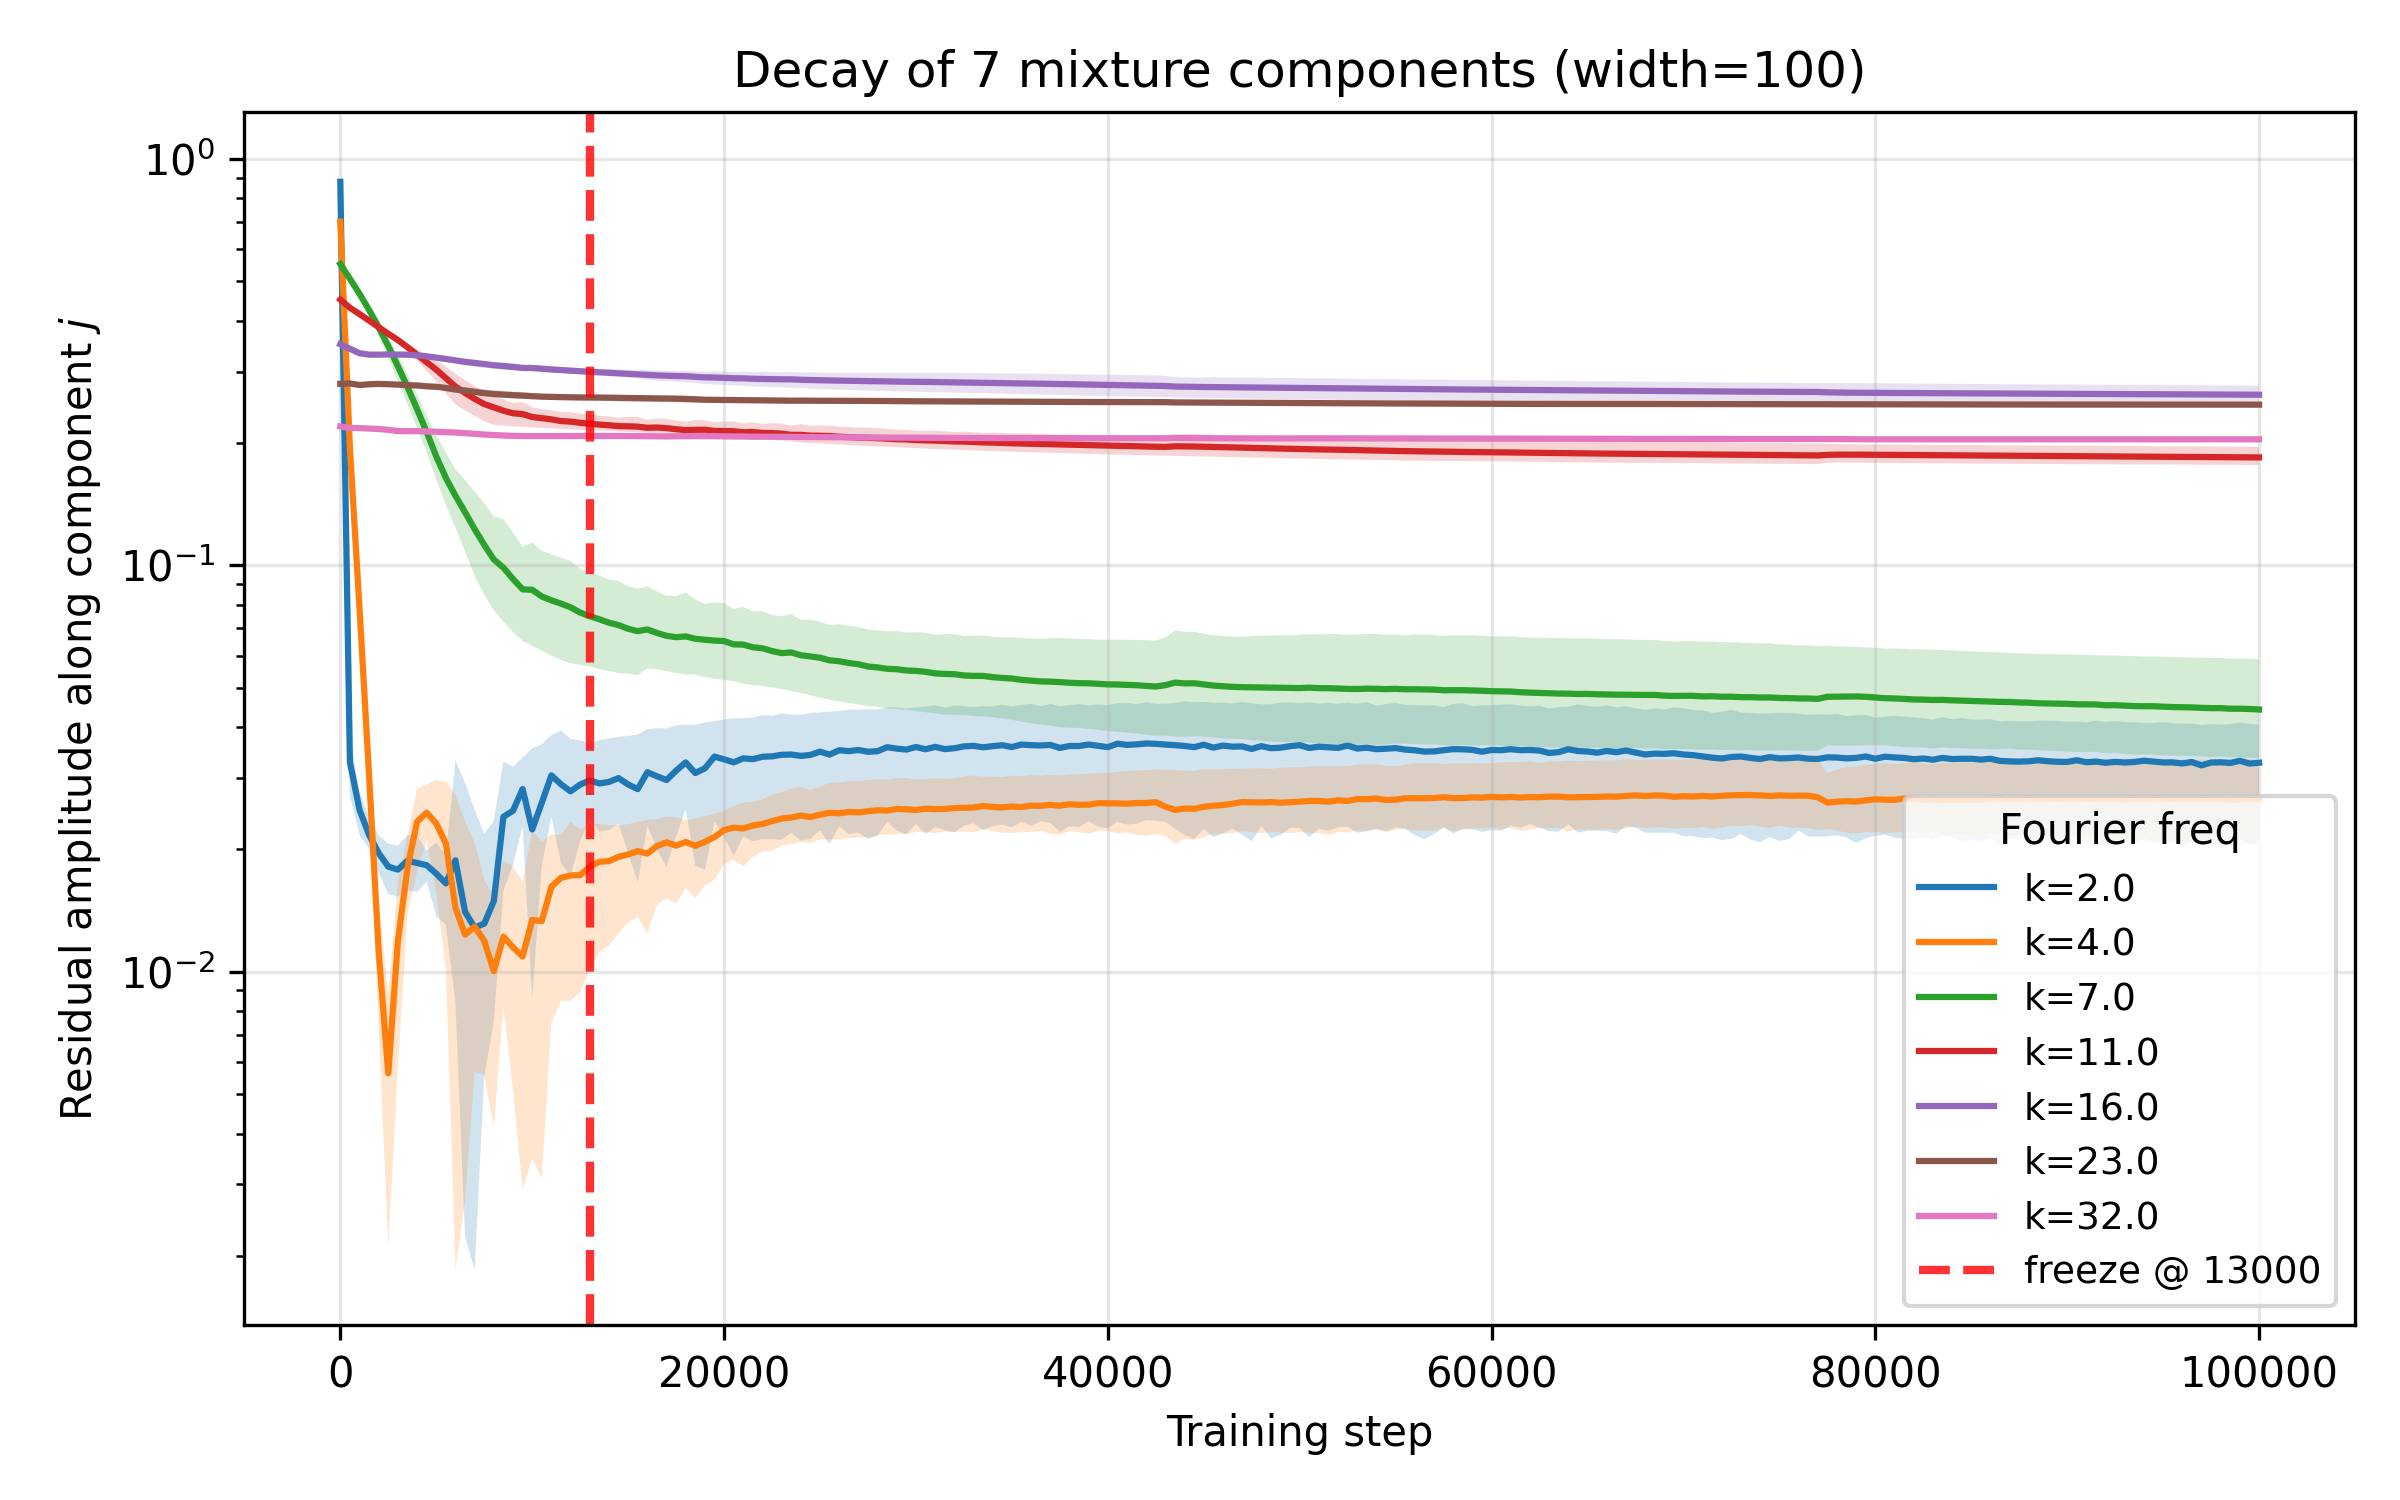
\includegraphics[width=.32\textwidth]{plots/fourier_decay/fourier_decay_w100} &
		
\includegraphics[width=.32\textwidth]{plots/fourier_decay/fourier_decay_w512} &
		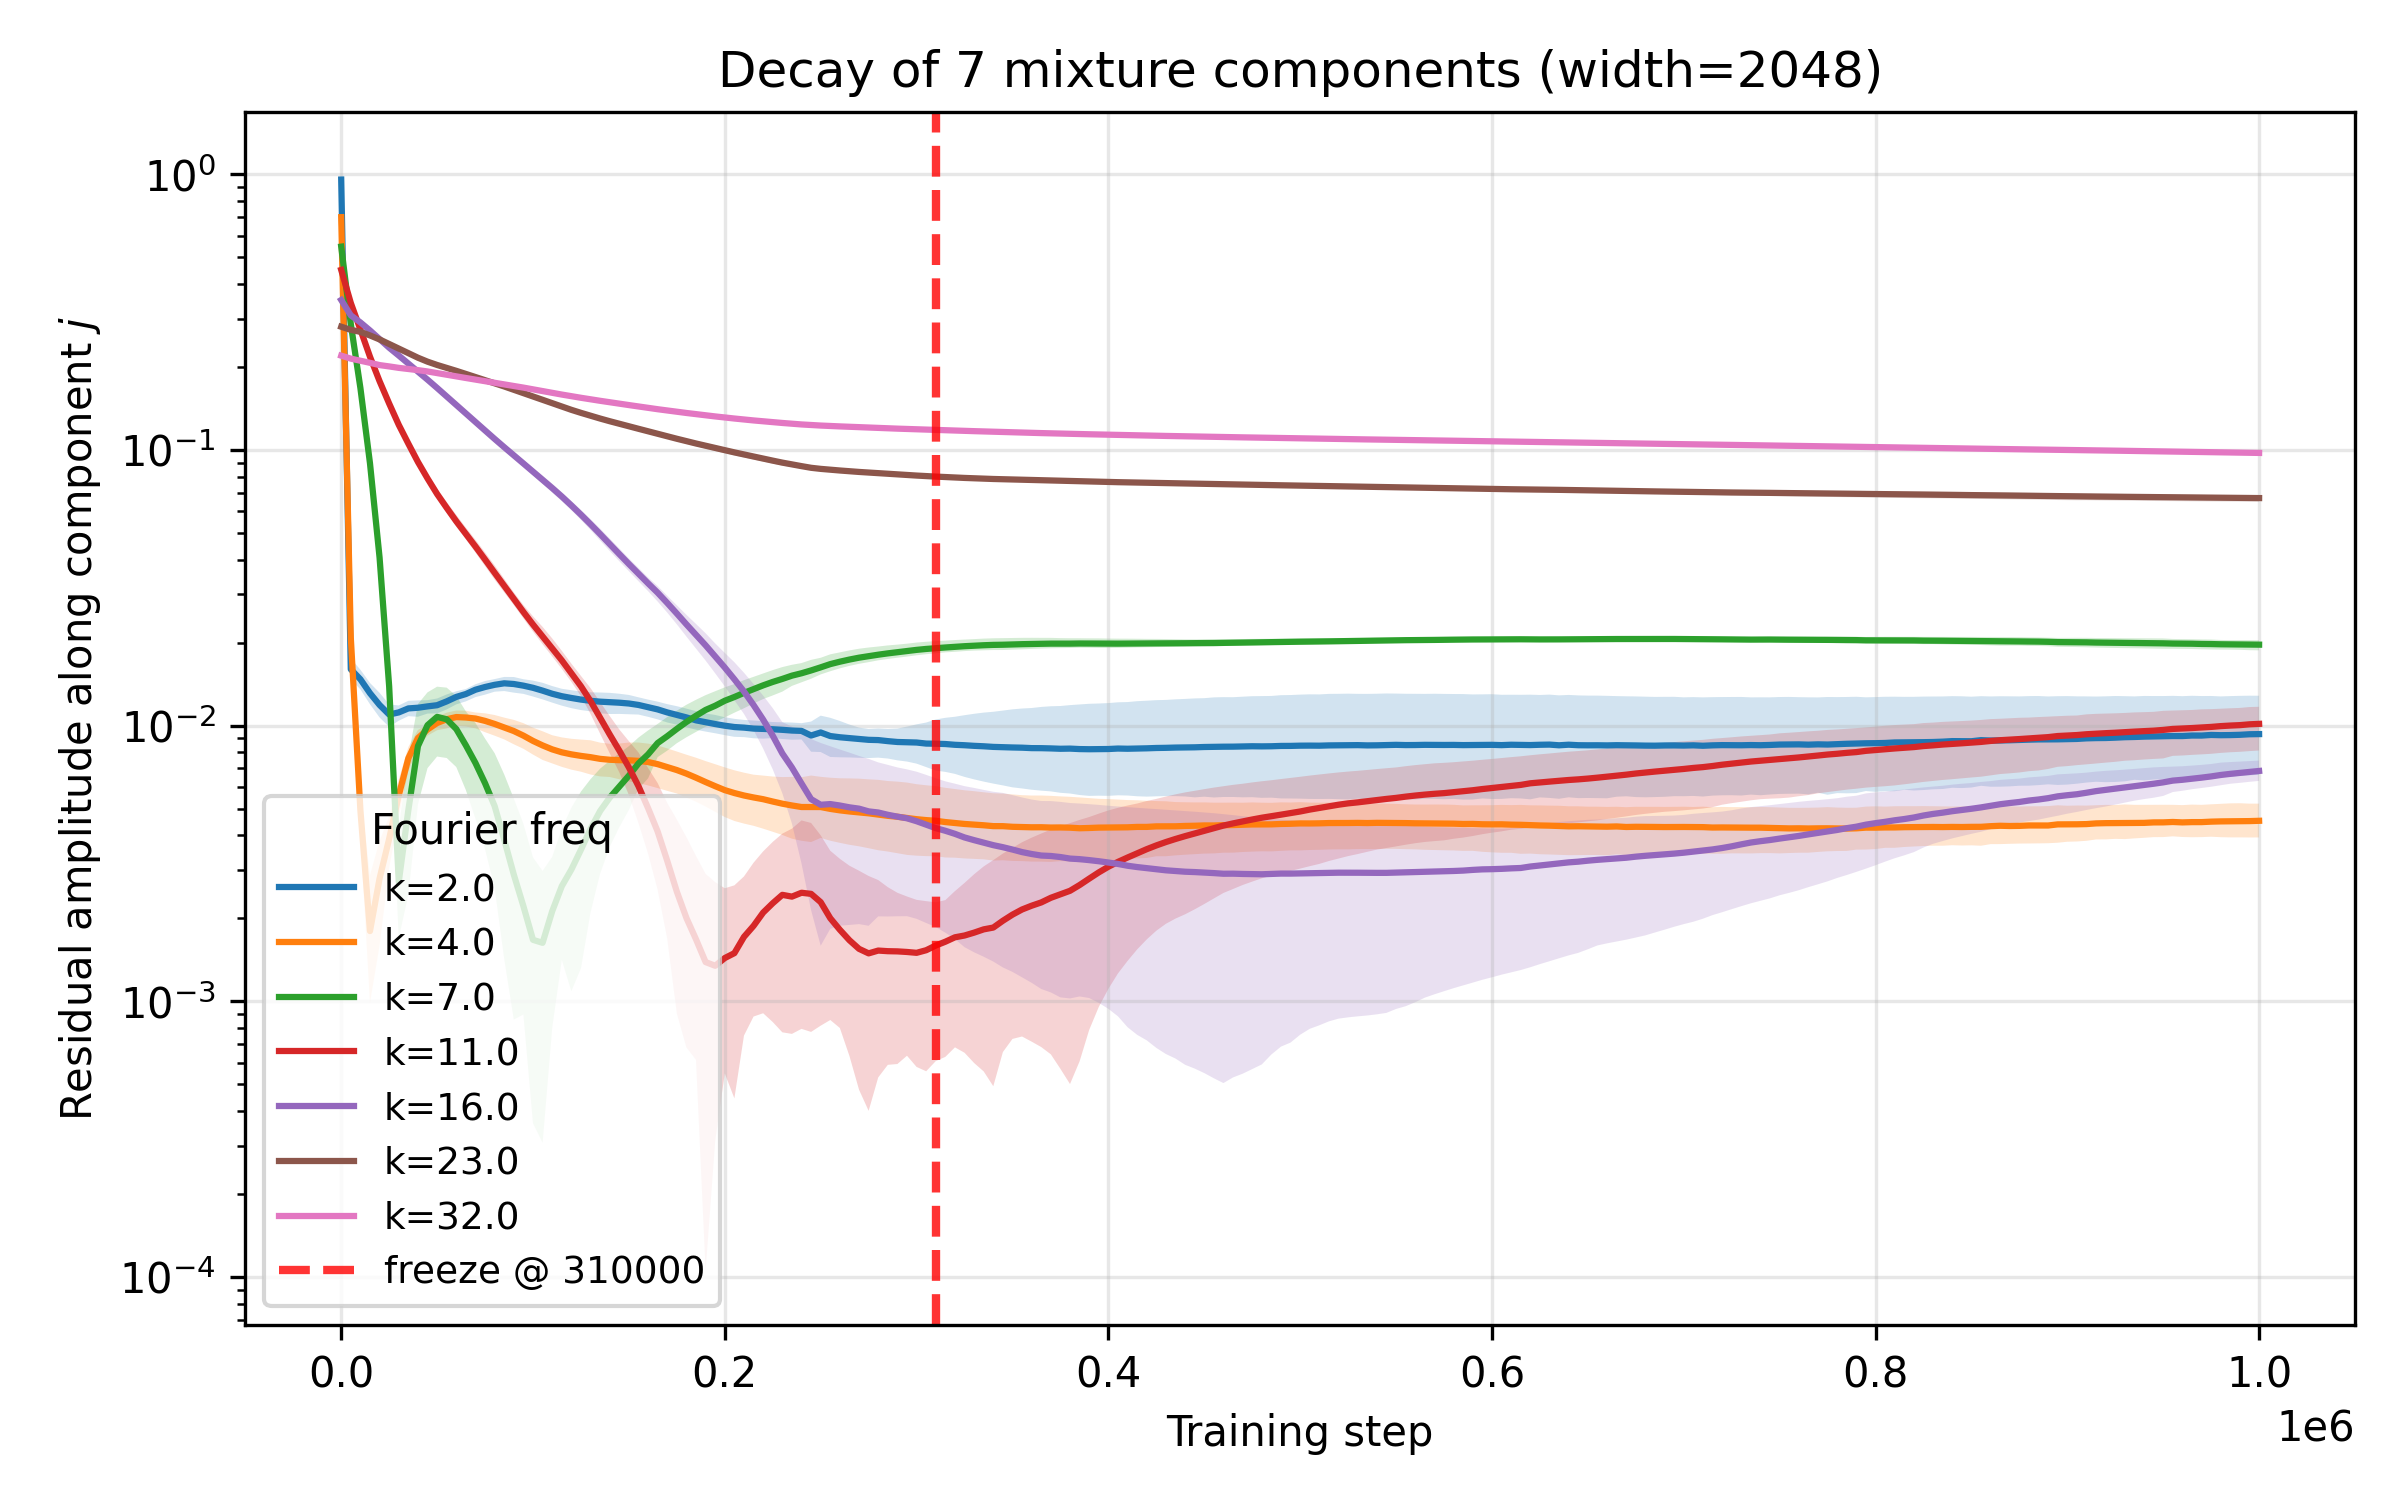
\includegraphics[width=.32\textwidth]{plots/fourier_decay/fourier_decay_w2048}                                               \\
		\small (a) $m{=}100$                                                          & \small (b) $m{=}512$ & \small (c) $m{=}2048$
	\end{tabular}

	\vspace{0.4em}
	\textbf{Observation.}
	Low-frequency Fourier components decay rapidly, while high-frequency components
	persist for much longer across widths.

	\textbf{Interpretation.}
	This provides a direct, frequency-resolved signal of frequency bias and motivates
	Q1 (finite samples) and Q2 (finite width).

\end{frame}

\begin{frame}{Planned Timeline and Diagnostics}

	\begin{itemize}
		\item \textbf{February: Analytic groundwork (Q1)}
		      \begin{itemize}
			      \item Analytically derive the exact operator NTK operator and the convolution operator
			            $T$ for 2-layer ReLU network on $S^1$.
			      \item Formulate the finite-sample discretization $T_n$ and the induced
			            coupled Fourier-mode dynamics.
			      \item Identify diagnostic quantities: frequency component-wise residual decay and
			            off-diagonal coupling between frequencies.
		      \end{itemize}
		      \vspace{0.4em}
		\item \textbf{March: Finite-sample experiments (Q1)}
		      \begin{itemize}
			      \item Simulate discretized kernel dynamics for varying sample sizes $n$.
			      \item Measure effective decay rates for each frequency component.
			      \item Quantify deviations from ideal exponential decay and onset of frequency coupling.
		      \end{itemize}
		      \vspace{0.4em}

	\end{itemize}

\end{frame}

\begin{frame}{Planned Timeline and Diagnostics}
	\begin{itemize}
		\item \textbf{April: Finite-width experiments (Q2)}
		      \begin{itemize}
			      \item Sweep network width $m$ with effectively infinite samples based
			            on results obtained from Q1, with fixed learning rate and training time.
			      \item Track residual coefficients of each frequency component across seeds.
			      \item Measure coupling of the frequency-components.
		      \end{itemize}
		      \vspace{0.4em}
		\item \textbf{April final weeks: Integration and write-up}
		      \begin{itemize}
			      \item Compare finite-sample and finite-width effects on frequency dynamics.
			      \item Consolidate results, refine figures, and finalize thesis chapters.
		      \end{itemize}

	\end{itemize}
\end{frame}

\begin{frame}{Thank you}
	Questions?
\end{frame}

% -----------------------
\end{document}
